\documentclass[tikz,border=5]{standalone}
\usetikzlibrary{positioning,decorations.pathreplacing}
\begin{document}

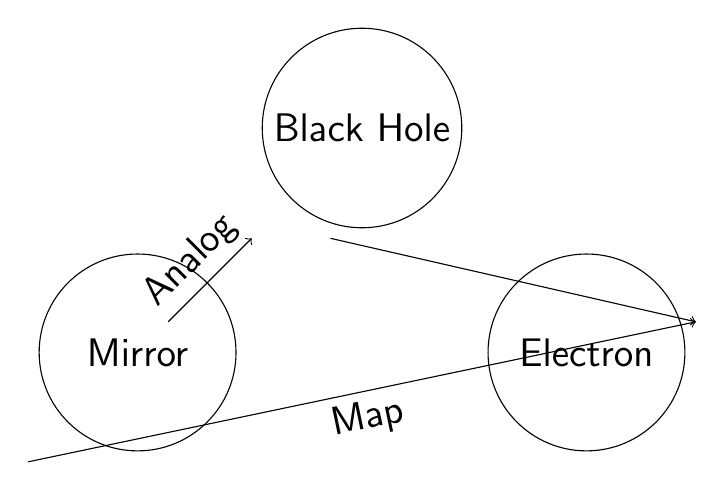
\begin{tikzpicture}[node distance={15mm},font=\sffamily\Large]
\node[circle,draw,minimum size=25mm](blackhole){Black Hole};
\node[circle,draw,minimum size=25mm,below left=of blackhole](mirror){Mirror};
\node[circle,draw,minimum size=25mm,below right=of blackhole](electron){Electron};
\draw[->] ([xshift=-5mm,yshift=-5mm]mirror.north east)--([xshift=-5mm,yshift=-5mm]blackhole.south west)node[midway,above,sloped]{Analog};
\draw[->] ([xshift=5mm,yshift=-5mm]blackhole.south west)--([xshift=5mm,yshift=-5mm]electron.north east)node[midway,above,sloped]{{}};
\draw[->] ([xshift=-5mm,yshift=-5mm]mirror.south west)--([xshift=5mm,yshift=-5mm]electron.north east)node[midway,below,sloped]{Map};
\end{tikzpicture}

\end{document}